\documentclass[final,hyperref={pdfpagelabels=false}]{beamer}
\mode<presentation>
{
  \usetheme{UNM}
}
  \usepackage{times}
  \usepackage{bm}
  \usepackage{ragged2e}
  \usepackage[numbers]{natbib}
  \usepackage{amsmath, amsthm, amssymb, latexsym}
  \boldmath
  \usepackage[english]{babel}
  \usepackage[latin1]{inputenc}
  \usepackage[orientation=portrait,size=a0,scale=1.4,debug]{beamerposter}
  \usepackage{tikz}
  \usepackage[linesnumbered,ruled,vlined]{algorithm2e}
  \usepackage{stmaryrd}
  \usepackage{floatrow}
  \usepackage{wrapfig}
  \usepackage{float}



\def\mbf{\mathbf}
\def\mc{\mathcal}
\def\msf{\mathsf}
\def\argmin{\mathop{\mathrm{argmin}}}
\def\sgn{\mathop{\mathsf{sign}}\nolimits}

  \graphicspath{{./figures/}}   
  \setbeamertemplate{itemize item}{\raisebox{0.1ex}{$\blacksquare$}\hskip0.1em}
  \renewcommand{\raggedright}{\leftskip=0.5cm \rightskip=0.5cm plus 0cm}
  \newcommand{\trace}[1]{\mbox{Tr($#1$)}}
  \providecommand{\e}[1]{\ensuremath{\times 10^{#1}}}
  \usetikzlibrary{shapes,snakes}
  \usetikzlibrary{arrows,calc,fadings,decorations.pathreplacing,positioning}
  \usetikzlibrary{automata}
  % Define box and box title style
  \tikzstyle{mybox} = [draw=contCol!90, fill=patCol!50, very thick,
  rectangle, inner sep=10pt, inner ysep=14pt]
  \tikzstyle{fancytitle} =[fill=contCol!70, text=black, draw=contCol!90, rectangle,
  sharp corners, font=\footnotesize\sf]
  \tikzset{
    blob/.style={
      circle,
            draw=black, thin,
            fill=patCol,
            minimum height=0.07em,
            minimum width=0.07em,
            text centered},
          punkt/.style={
            rectangle,
            draw=black, thin,
            fill=contCol!60,
            minimum height=0.1em,
            minimum width=0.1em,
            text centered},
          % Define arrow style
          pil/.style={
            ->,
            >=stealth,
            thin,
            shorten <=1pt,
            shorten >=1pt,}
        }
\tikzstyle{every picture}+=[remember picture]
\tikzstyle{na} = [baseline=-.5ex]

  %%%%%%%%%%%%%%%%%%%%%%%%%%%%%%%%%%%%%%%%%%%%%%%%%%%%%%%%%%%%%%%%%%%%%%%%%%%%%%%%%5
\title[Fancy  Posters]{Successfully learning networks from undersampled neuroimaging data}  
\author[Plis et
al.]{D. Danks, S.M. Plis, C. Freeman, A. Caprihan, Eswar Damaraju, V. D.  Calhoun} \institute[]{  Carnegie Mellon University,  The
  Mind Research Network}
  %\date{}

  %%%%%%%%%%%%%%%%%%%%%%%%%%%%%%%%%%%%%%%%%%%%%%%%%%%%%%%%%%%%%%%%%%%%%%%%%%%%%%%%%5
  \begin{document}
  \begin{frame}{} 
    \begin{columns}[t]
      \begin{column}{.48\linewidth}
        \begin{block}{\Large Abstract}
          \raggedright 
          \begin{itemize}
            \item Many structure learning algorithms are based on Granger causality
            \item Granger causality is unreliable given undersampled time series data
            \item We developed RASL to learn structure from undersampled data
            \item In simulated data, RASL algorithms reveal causal timescale structure 
              and improved measurement timescale learning 
            \item RASL algorithms provide additional insight on fMRI data
          \end{itemize}
          
          
        \end{block}

        \begin{block}{\Large Problems with ``Granger Causality''}
          \raggedright 
          \begin{itemize}
          \item \textbf{Granger causality}: $X$ Granger-causes $Y \equiv$ $X$'s 
          history provides information about $Y$'s current state (beyond $Y$'s history)
          
          \item Mathematically: $Y^t = \sum_{i=1}^k \big[ \alpha_i Y^{t-i} + \beta_i X^{t-i} \big]$
          is a significantly better predictor of $Y^t$ than
          $Y^t = \sum_{i=1}^k \alpha_i Y^{t-i}$ (perhaps with covariates)
           
          \item Granger causality only reliable if key assumptions hold:
          \begin{itemize}
            \item \emph{Linearity} (but hemodynamic convolution does not create problems)
            \item \emph{Causal sufficiency} (but becoming less of a problem)
            \item \emph{Equal timescales} for both measurement and underlying causation
            \end{itemize}
           
          \item \textbf{Undersampling}: Measurement timescale significantly slower than
          causal or communication timescale 
          \begin{itemize} \item Intermediate time points are unobserved \end{itemize} %figure here that sergey wants
          
          \includegraphics[scale = 2.1]{undersample}

          \item Granger causality can be arbitrarily wrong given undersampling
          \begin{itemize}
            \item $X$ GC $Y$ even though $Y$ actually causes $X$
            \item $X$ GC $Y$ even though no direct causal connection
            \item $X$ doesn't GC $Y$ even though $X$ actually causes $Y$
            \end{itemize}
          
          \item Undersampling is a ubiquitous, persistent feature of fMRI data
          
          \item \textbf{Conclusion}: Structure learning algorithms based on Granger causality
          are likely unreliable given fMRI data
          \end{itemize}
        \end{block}

        \begin{block}{\Large How to Overcome the Problems}
          \begin{minipage}{0.5\textwidth}
            %\raggedleft
            \vspace{10 mm}
            \LinesNumberedHidden
            \SetKwProg{myalg}{Algorithm}{}{}
            \myalg{RecursiveEqClass}{

            \KwIn{${\cal H}$}
            \KwOut{$\llbracket{\cal H}\rrbracket$}

            initialize empty graph ${\cal G}$
            and set $S$

            \BlankLine
            \Begin($EdgeAdder$ $ {\cal G}^*, {\cal H}, L $) {
              \If{$L$ has elements}
              {
                \ForAll{edges in $L$}{
                  \If{edge creates a conflict}
                  { remove it from $L$ }
                }
                \If{$L$ has elements}
                {
                  \ForAll{edges in $L$}{
                    add the edge to ${\cal G}^*$

                    \If{$\exists {\cal G} \in \{({\cal G}^*)^u\} \text{ s.t. } {\cal
                        G} = {\cal H}$}
                    { 
                      add ${\cal G}^*$ to $S$
                    }
                    $EdgeAdder$ ${\cal G}^*, {\cal H},
                    L\setminus\text{the edge}$

                    remove the edge from ${\cal G}^*$
                  }
                }
                
              }
            }

            \BlankLine
            put all $n^2$ edges into list $L$

            $EdgeAdder({\cal G},{\cal H}, L)$

            \Return $S$
          }
        \end{minipage} %
        \begin{minipage}{0.4\textwidth}
          \centerline{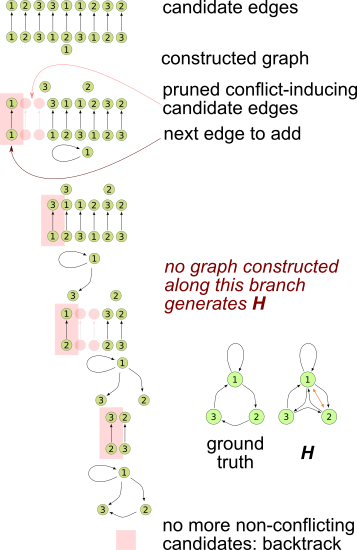
\includegraphics[scale = 1.8]{recursive_tree}}
          %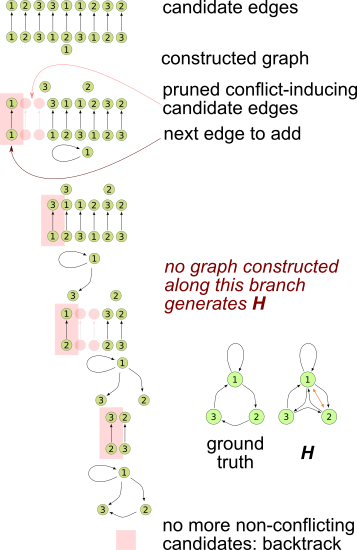
\includegraphics[width=\linewidth]{recursive_tree}
        \end{minipage}



        \begin{minipage}{.9\textwidth}
        \vspace{20 mm}
          Start with an empty graph and $n^2$  possible edges. For each edge $e$, construct a graph ${\cal G}$ containing only $e$. If ${\cal G}^{u} \nsubseteq {\cal  H}$  for all $u$, then reject; else if ${\cal G}^{u} = {\cal  H}$ for some $u$, then add ${\cal G}$ to $\llbracket{\cal H}\rrbracket$; else, recurse into non-conflicting graphs in order.
        \end{minipage}% 
        \end{block}
  
  

      \end{column}
      %%%%%%%%%%%%%%%%%%%%%%%%%%%%%%%%%%%%%%%%%%%%%%%%%%
      \begin{column}{.48\linewidth}


        \begin{block}{\Large Synthetic Data}
        %\raggedright
          \begin{minipage}{1\textwidth}
          %\includegraphics[scale = 1.1]{fig9_MSL}
          \includegraphics[scale = 2.2]{fig9_MSL_transparent}
        \end{minipage} %

        \begin{minipage}{.95\textwidth}
        \vspace{5 mm}
           Graphs with $15$, $20$ ,$25$, $30$, and $35$ nodes at the density of $10\%$, their corresponding ${\cal G}^{2}$ and equivalence class size distribution as well as the running time summarizing the computation of $100$ random SCCs per node size
        \end{minipage}% 

        \begin{minipage}{1\textwidth}
                \vspace{5 mm}
          %\includegraphics[scale = 1.57]{figure_6_RASL}
          \includegraphics[scale = 2]{figure_6_RASL_transparent}
        \end{minipage} %

        \begin{minipage}{.95\textwidth}
        \vspace{5 mm}
           The above plots the size of $\llbracket{\cal H}\rrbracket$ as a function of $u$ for $100$ random $5$-node SCCs with $25\%$ density,  each  of  which   was undersampled  for $u \in \{ 2 , \ldots , 11 \}$. 
        \end{minipage}% 
       
        \begin{minipage}{1\textwidth}
                \vspace{5 mm}
          %\includegraphics[scale=1.07]{RASL_simulations_6nodes_u2}
          \includegraphics[scale=1.27]{RASL_simulations_6nodes_u2_transparent}

        \end{minipage} %

        \begin{minipage}{.95\textwidth}
        \vspace{5 mm}
           The estimation and search errors on synthetic data undersampled at rate $2$. 
        \end{minipage}% 
        \end{block}

        \begin{block}{\Large Conclusions}
          \raggedright We have shown that undersampling leads to incorrect estimation of causal interactions. We have solved the forward problem and provided methods to generate undersampled graph from the ground truth. More importantly, we have solved the inverse problem and provided efficient algorithms both for known and unknown undersampling rates.  We discovered that very often equivalence classes of estimated graphs often are singletons - a useful property for post-hoc results analysis in practical applications. We have evidence that our method can further be used to correct  statistical estimation errors in standard within time-scale algorithms.
        \end{block}
        \begin{block}{References}
          \raggedright
          \footnotesize
          \begin{thebibliography}{2}
            \raggedright
          \bibitem
             GGranger, C.W.J.
            \newblock Investigating causal relations by econometric models and cross-spectral methods.
            \newblock In \emph{Econometrica}, 37(3), 424-438,1969.
          \bibitem
             PPlis S.M., Danks D., Yang J.
            \newblock Mesochronal structure learning
            \newblock In \emph{Proceedings of the Thirty-First Conference Annual Conference
  on Uncertainty in Artificial Intelligence (UAI-15)}, 2015.
          \end{thebibliography}
        \end{block}
      \end{column}
    \end{columns}
  \end{frame}
\end{document}


%%%%%%%%%%%%%%%%%%%%%%%%%%%%%%%%%%%%%%%%%%%%%%%%%%%%%%%%%%%%%%%%%%%%%%%%%%%%%%%%%%%%%%%%%%%%%%%%%%%%
%%% Local Variables: 
%%% mode: latex
%%% TeX-PDF-mode: t
%%% End:
